\subsection{Mikrocontroller} \label{sec:microcontrollerHardware}

Als Microcontroller wurde ein nRF52832 der Firma Nordic Semiconductors verwendet ( ersichtlich in Abbildung \ref{fig:nRF52832}). Seine hohe Performance ermöglicht es ein System aufzubauen, welches den Microcontroller als zentrale Schnittstelle beinhaltet. Der Microcontroller bildet wie in Kapitel \ref{sec:gesamtkonzept} gemäss Abbildung \ref{fig:Teilsysteme} bereits beschrieben das Herzstück des Dōjōs. 

\begin{figure}[H]
	\begin{center}
		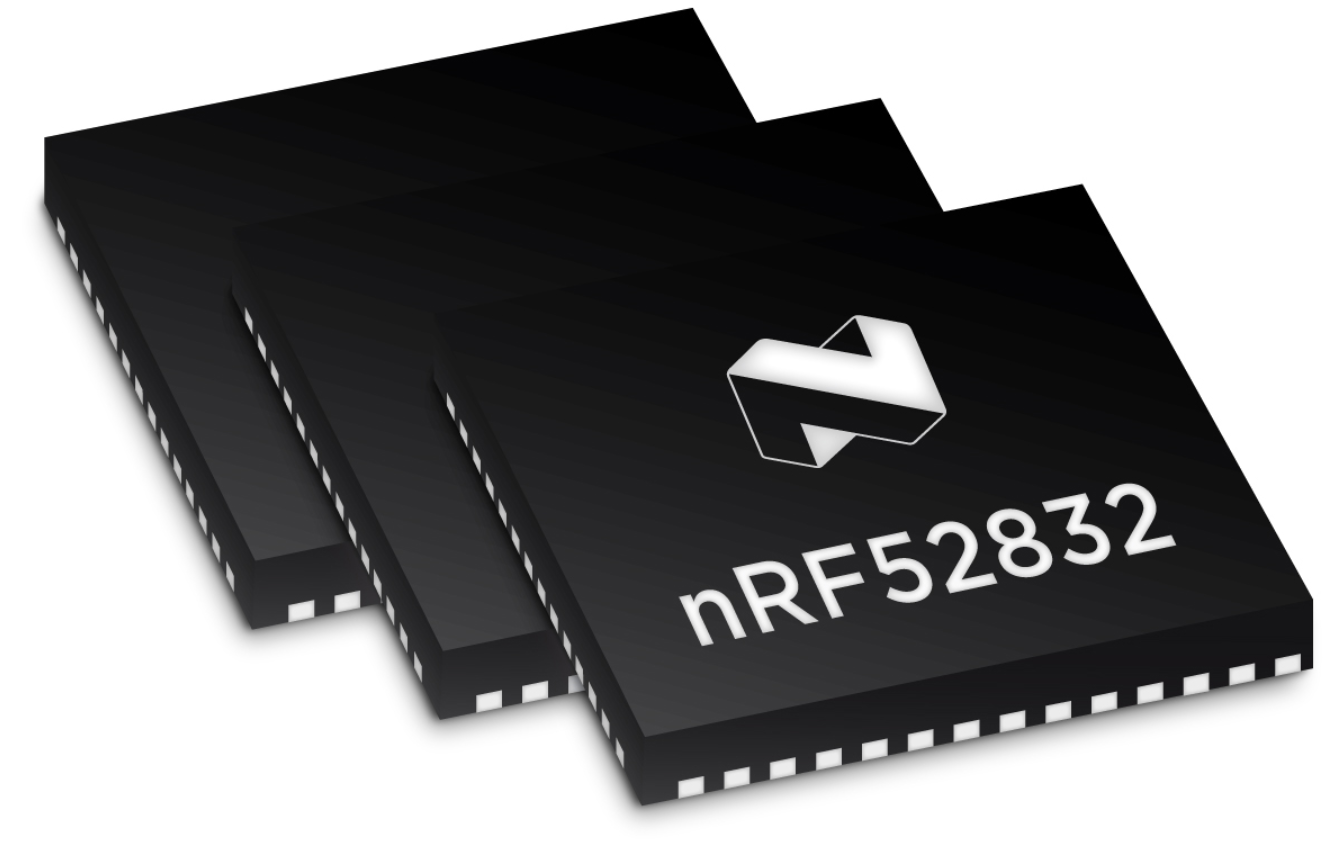
\includegraphics[width=60mm]{data/nRF52832.png}
		\caption[nRF52832 Microcontroller]{nRF52832 Microcontroller \cite{nRF52832}} %picture caption
		\label{fig:nRF52832}
	\end{center}
\end{figure}

der nRF52832 weist eine Betriebsversorgungsspannung zwischen 1.7V und 3.6V mit einem Versorgungsstrom von 5.4mA auf. Der Speicher des nRF52832 ist durch 512kB flash/64kB RAM Speicher gegeben. 
Für die ersten Tests der Software wurde ein Development Kit (Abbildung \ref{fig:nRF52832-DK}) mit intergriertem nRF52832 verwendet. Die Beschreibung der Software ist in Kapitel \ref{sec:software} ersichtlich.
\begin{figure}[H]
	\begin{center}
		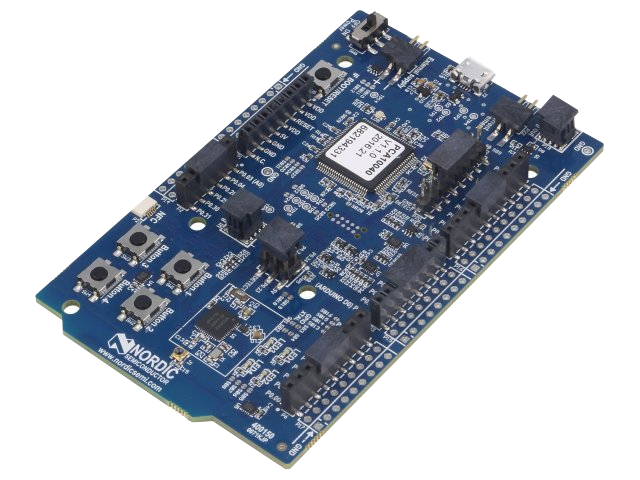
\includegraphics[width=100mm]{data/NRF52-DK.png}
		\caption[nRF52 Development Kit]{nRF52 Development Kit \cite{nRF52-DK}} %picture caption
		\label{fig:nRF52832-DK}
	\end{center}
\end{figure}
 Die Schlüsselmerkmale dieses Boards sind zum einen wie bereits beschrieben der integrierte Microcontroller, zum anderen aber auch eine integrierte Bluetooth Antenne. Das Kit unterstützt proprietäre Bluetooth Smart, ANT und 2.4GHz Applikationen. Zudem ermöglicht es den Einsatz von Drittanbieter Shields. Dies ermöglicht das Beschreiben und Lesen der SD-Karte zu testen.
